%Task 8
\newpage

\section*{Task 7}

In this task we're asked to implement one syncronomous, and one asynchronous 3-bit counter, and contrast them.

\subsection*{Asynchronous counter}
\begin{figure}[H]
    \begin{centering}
    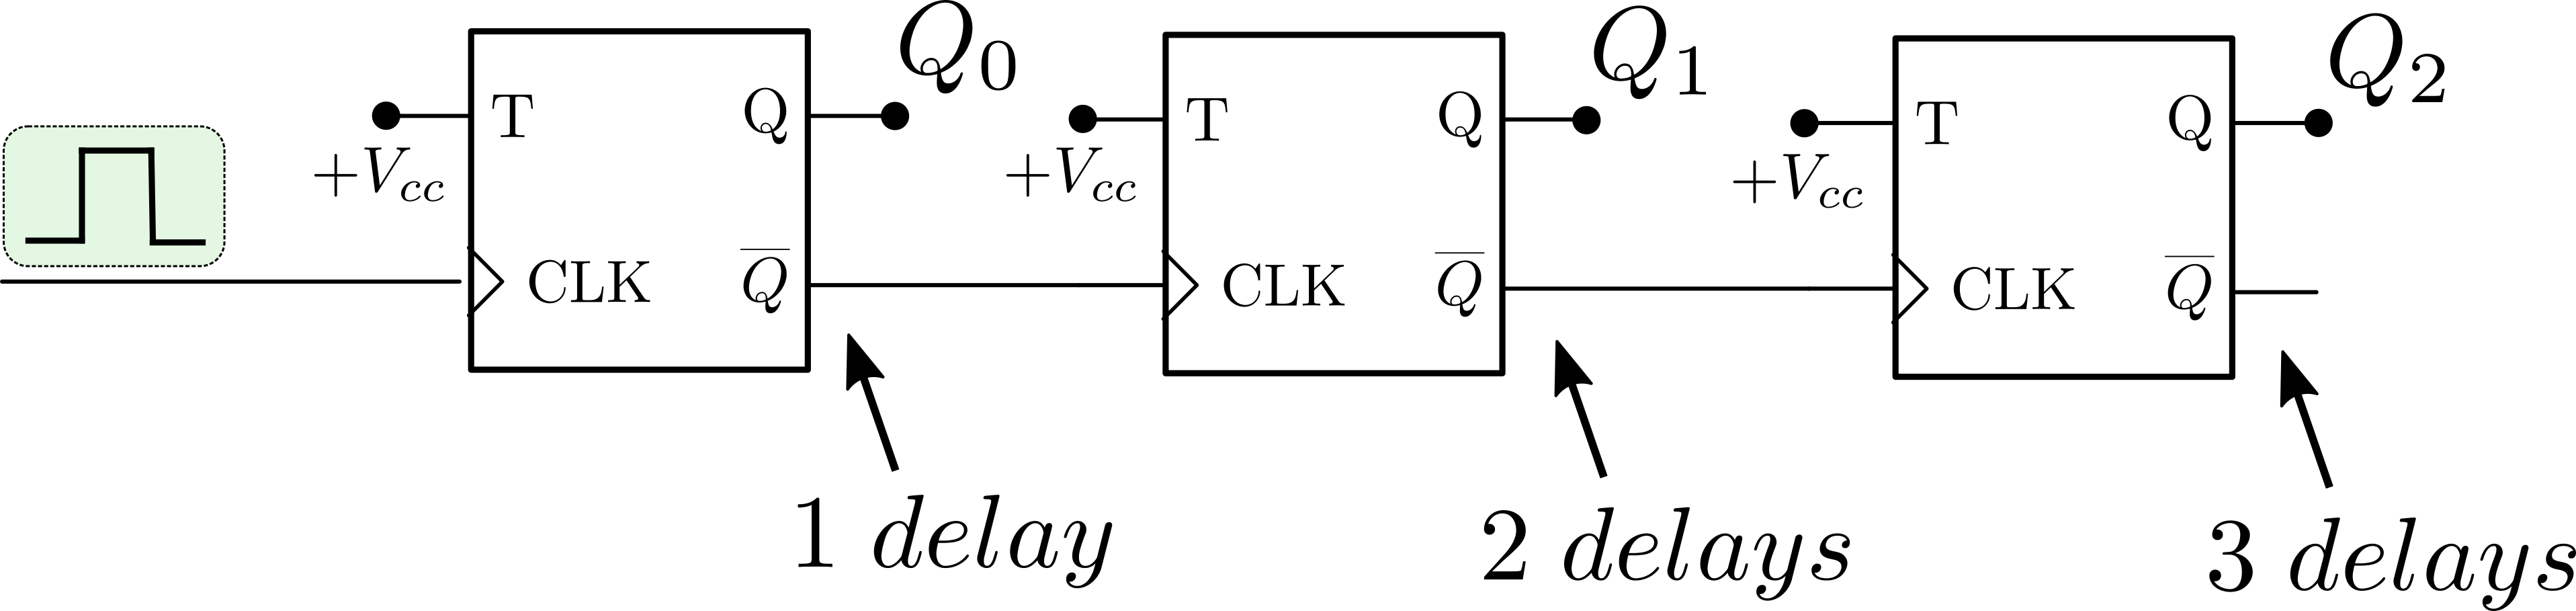
\includegraphics[width=1\textwidth]{data/async.png}
    \par\end{centering}
    \caption{Async. counter - delays}
\end{figure}


This counter work with a casquade triggering flip flops clocks done by the not Q output.

The idea is that, everytime the left flip flop is clocked two times, not Q goes up one time, thus, right flip flop is clocked one time (the half)
Propagating this logic to the general case, n-th flip flop has a period $2^n$ thus we made a binary counter. 

The theorical problem of this system is the delay propagation. As there is a delay between clock rising edge and Q update, the total delay will be multiplied by the number of flip flops.

\subsection*{Synchronous counter}
\begin{figure}[H]
    \begin{centering}
    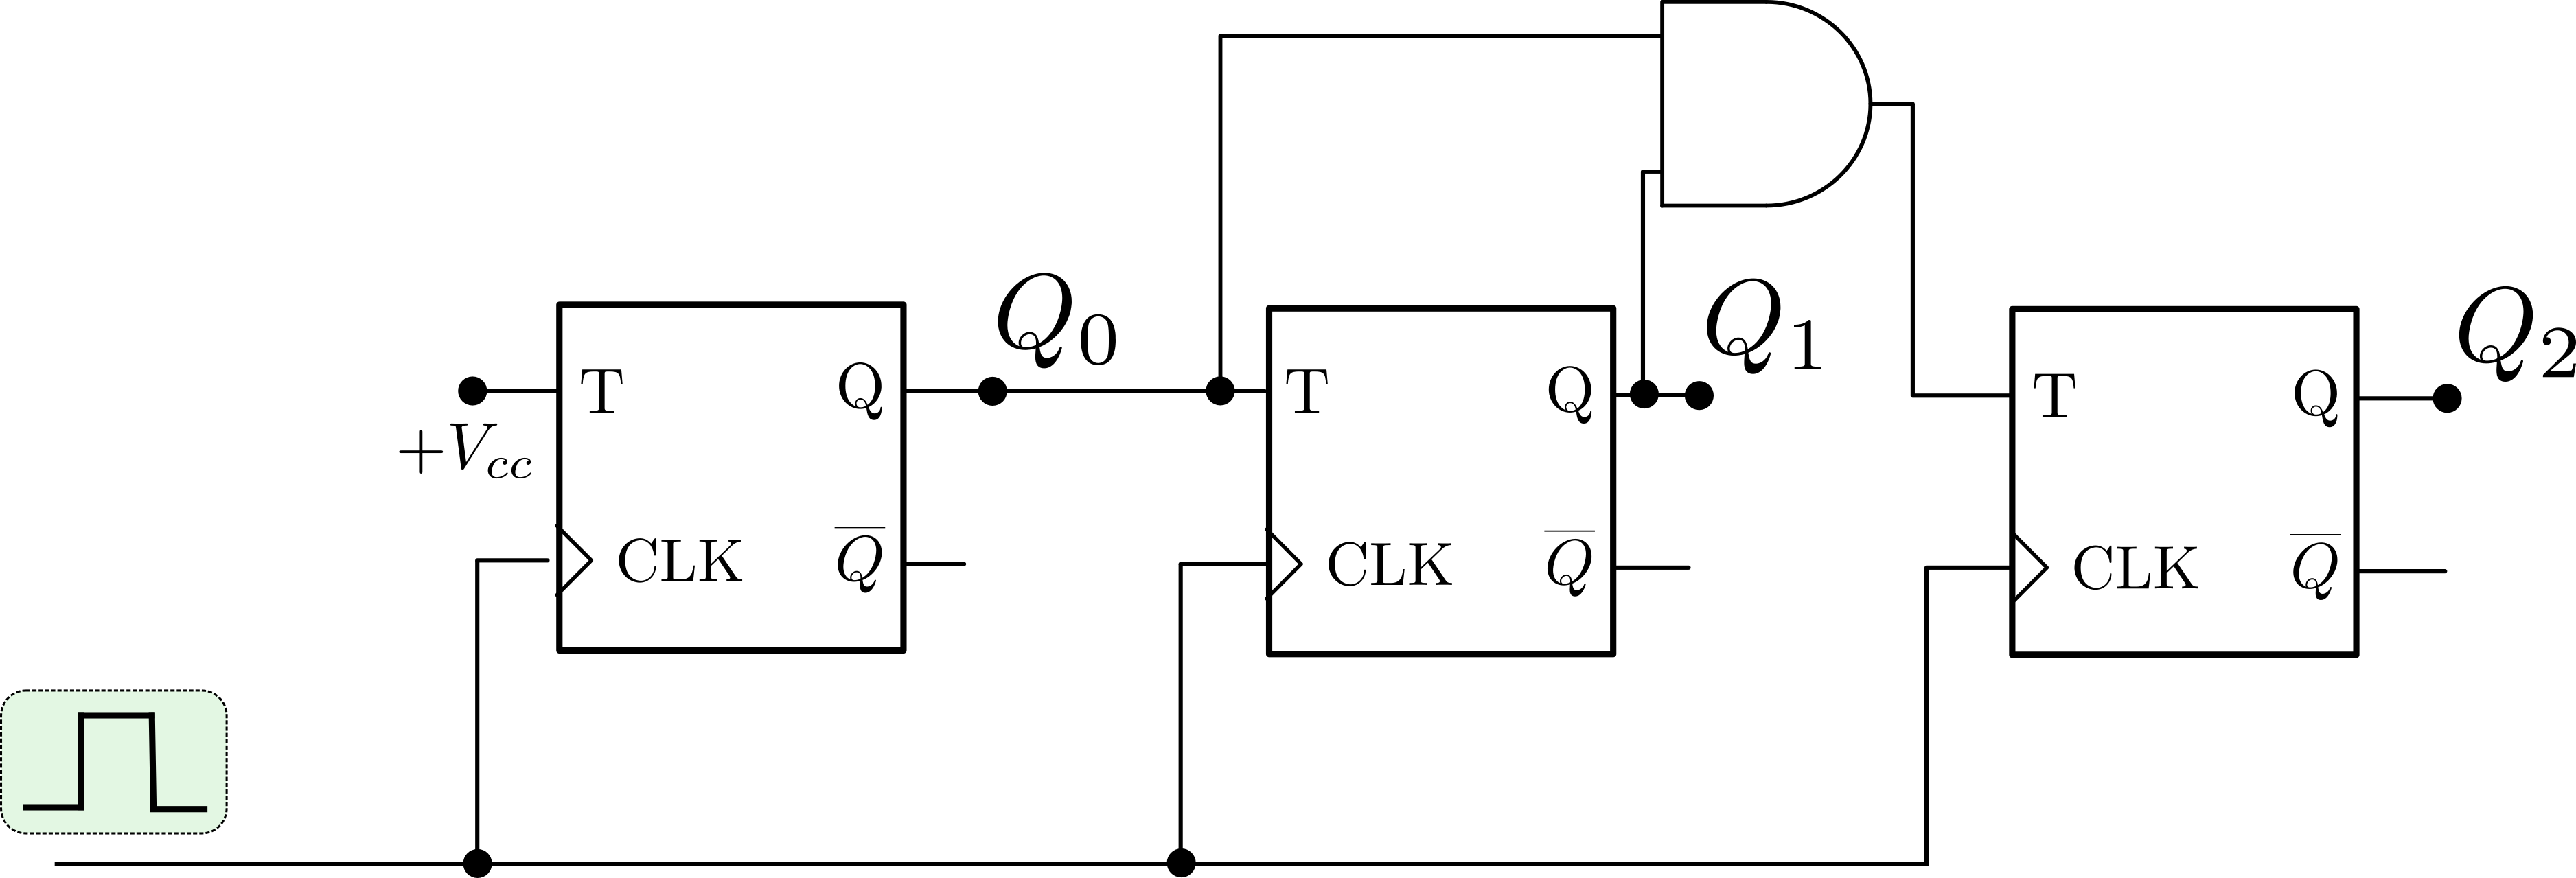
\includegraphics[width=1\textwidth]{data/sync.png}
    \par\end{centering}
    \caption{Sync. counter - delays}
\end{figure}

This counter is made to fix the problem of the previous counter. In this logic, all flip flops clocks are connected to the same trigger, thus, all of them are updated in the same instant, not, one after the other. We control if each flip flop switches by controlling the T input. Flip flop 2 needs flip flop 1 to be in 1 to switch (01->10). Flip flop 3 needs both previous two flip flops in 1 to switch. (011->100)

\subsection*{Measurements}

We built the counters for both cases. As expected, in low frequencies diferences weren't noticed. But, when we increased frecuency to 1Mhz at clock input we were able to see a difference

\begin{figure}[H]
    \begin{centering}
    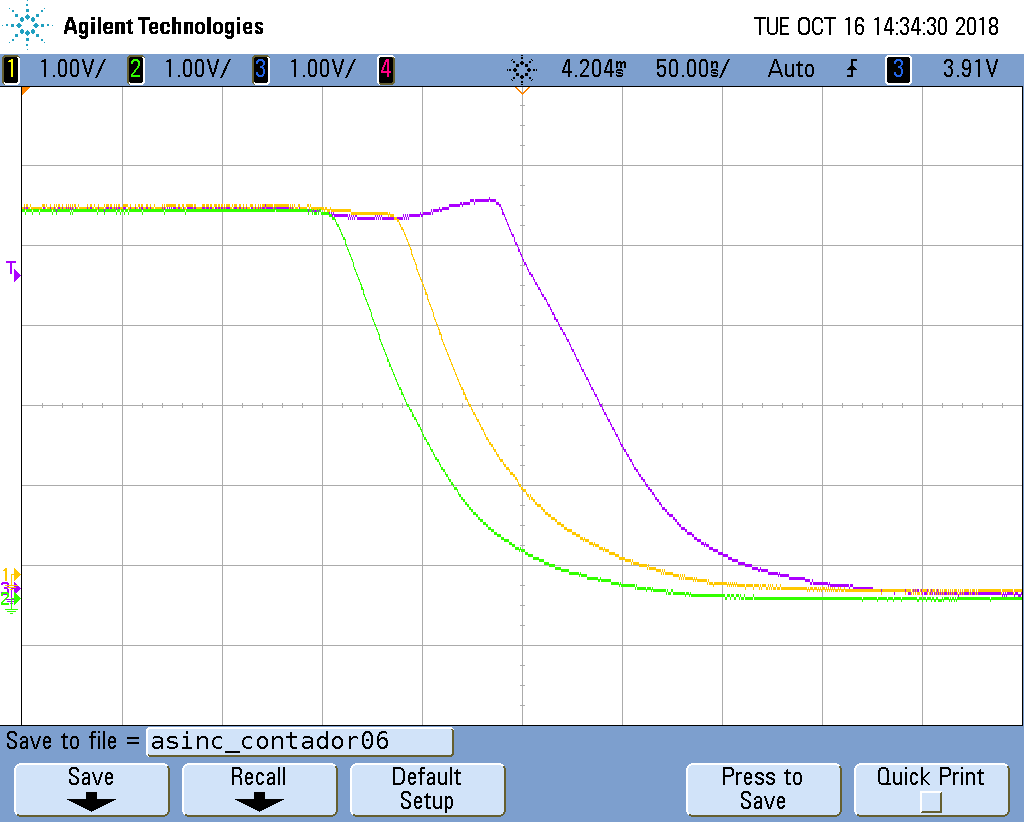
\includegraphics[width=0.45\textwidth]{data/asinc_contador06.png}
    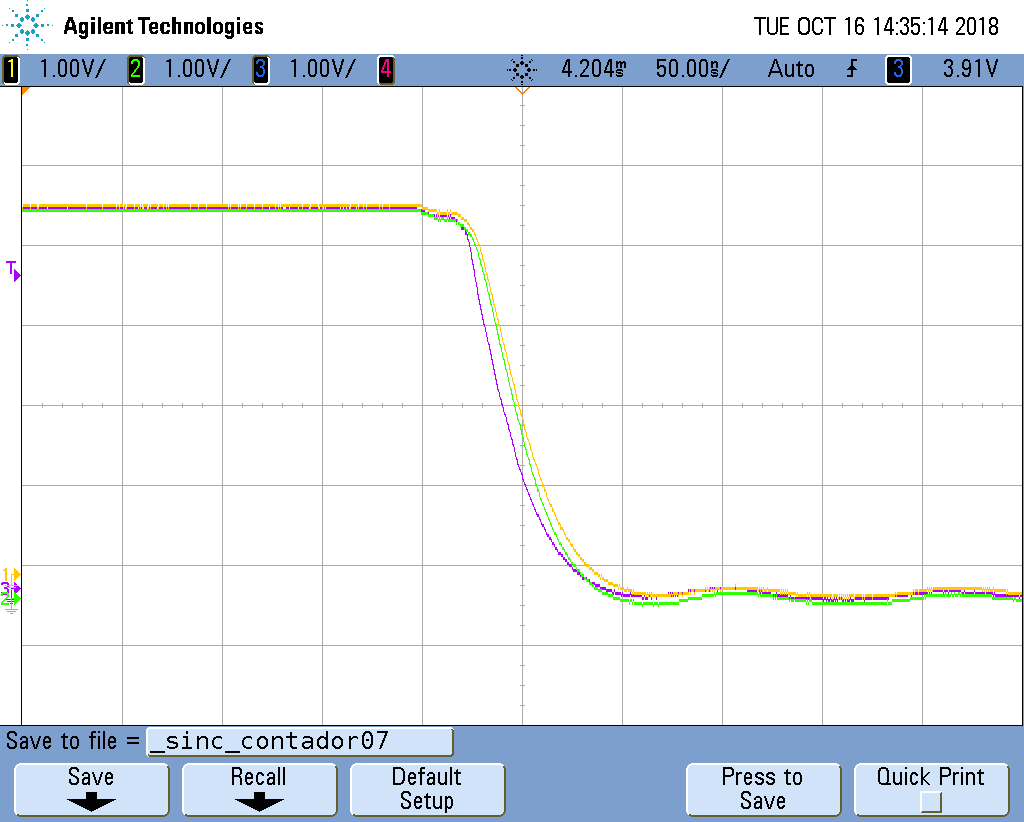
\includegraphics[width=0.45\textwidth]{data/_sinc_contador07.png}
    \par\end{centering}
    \caption{Comparison - 1Mhz clock - $Q_0$,$Q_1$,$Q_2$ signals - async, sync counters, left to right}
\end{figure}

From figure we can see that in async circuit bits are updated one after the other, while in sync circuit all of them are updated at the same time.
Also we should note that updates are not instant, as it was assumed in previous analisis. There is countinous change, that creates an evident limitation to circuit.
This limitation made both counters unusable with frecuencies slighty higher than 1Mhz (1Mhz was the higher frecuency with proper functioning found in both cases), cause the flip flops were switched before the output signal reached its corresponding logic level.
So, with 3 bits in practice there is no difference between both circuits, as this limitation impacts both circuits in, apparently, the same way.

